\message{ !name(main.tex)}
%%%
% Any line that begins with a percent symbol is a comment. To compile
% this document and view the output:
%
% Run Latex
% Run Bibtex
% Then run Latex twice.
%
% This should produce the output PDF file named main.pdf
%%%

% This defines the style to use for this document.
% Do not modify.
\documentclass[letterpaper]{article}

% The following are akin to "import" statements in Python or Java -
% these import useful commands into the document for you to use.  You
% don't have to modify any of these lines. The AAAI package formats
% this document in the style of submissions to the American
% Association for Artificial Intelligence conference, one of the top
% AI conferences in the world. You will find that many academic
% publications in AI use this format.
\usepackage{aaai} 
\usepackage{times} 
\usepackage{helvet} 
\usepackage{courier} 
\setlength{\pdfpagewidth}{8.5in} 
\setlength{\pdfpageheight}{11in} 
\usepackage{amsmath}
\usepackage{amsthm}
\usepackage{graphicx}
\usepackage{graphics}
\usepackage{moreverb}
\usepackage{subfigure}
\usepackage{epsfig}
\usepackage{txfonts}
\usepackage{algpseudocode}
\usepackage{multirow, multicol}
\usepackage{url}
\usepackage{tablefootnote}
\usepackage{color}

\setcounter{secnumdepth}{1}
\nocopyright

% Fill in your paper title, names and emails below
% The "\\" is used to break lines. The \url command
% is useful for typesetting URLs and email addresses (it uses the
% Courier font).
\title{Predicting Wine Quality}
 \author{Mackenzie Carey \and Laura Hiatt\\
 \url{{macarey, lahiatt}@davidson.edu}\\
 Davidson College\\
 Davidson, NC 28035\\
 U.S.A.}

% This is the "true" start of the document. All the text in your
% write-up should be placed within the \begin{document} and
% \end{document} decorators.
\begin{document}

\message{ !name(main.tex) !offset(-3) }


\maketitle % formats the title nicely, do not modify

% While at this point you could just begin your write-up, often, it's
% useful to write each section of your write-up in a separate tex
% file (not unlike the modular decomposition you do for code you
% write). These \input commands insert the contents of the
% specified tex files in the order specified. Every write-up you
% submit must contain the following sections, in the shown order. Open
% each of the indicated tex files to understand what goes in each
% section, as well as for more TeX tips.

% Place the contents of your abstract between the
% \begin{abstract} and \end{abstract} decorators.

\begin{abstract}

The abstract should be between four and seven sentences long. Introduce the
problem you are studying. Describe what you did. Summarize your results --- what
did you discover, what is the main take-away message?) Basically, you're trying 
to sell your paper to the reader, so be brief and to the point. \textbf{Do \emph{not}
include any citations in the abstract.}

% The \textbf{} command makes the specified text bold. The \emph{} or
% \textit{} command are used to italicize text. In general, text is never
% underlined.

% DON'T FORGET TO MATCH EACH OPEN BRACE WITH A CLOSING BRACE!
\end{abstract}



% The \section{} command formats and sets the title of this
% section. We'll deal with labels later.
\section{Introduction}
\label{sec:intro}

Given a set of data points, regression in its simplest form attempts to 
determine a line of best fit to describe the relationship between both an
input and an output variable. However, a straight line may fail to
accurately represent the data. A better representation may be through
the form of a higher order polynomial. In our experiment, we utilize
a random search k-fold cross-validation implementation of stochastic
gradient descent to determine the relationship between 11 attributes of wine,
Figure \ref{tab:attributes}, and a quality score as determined by wine experts
between one and ten. The quality value being a sensory input based on taste
and the 11 attributes ones of scientific measure.



\begin{figure}[htb]
  \centering % centers the entire table

  % The following line sets the parameters of the table: we'll have
  % three columns (one per 'c'), each
  % column will be centered (hence the 'c'; 'l' or 'r' will left or
  % right justify the column) and the columns
  % will have lines between them (that's the purpose of the |s between
  % the 'c's).
  \begin{tabular}{|c|c|c|} 
    \hline \hline % draws two horizontal lines at the top of the table
    Feature \\ % separate column contents using the &
    \hline % line after the column headers
    $fixed \phantom aacidity$\\
    $volatile   \phantom  aacidity$\\
    $citric   \phantom aacid$\\
    $residual   \phantom ssugar$\\
    $chlorides$\\
    $free   \phantom ssulfur \phantom ddioxide$\\
    $total  \phantom ssulfur  \phantom ddioxide$\\
    $density$\\
    $pH$\\
    $sulphates$\\
    $alcohol$\\
    \hline \hline
  \end{tabular}

  % As with figures, *every* table should have a descriptive caption
  % and a label for ease of reference.
  \caption{An example table.}
  \label{tab:attributes}
\end{figure}

In this section, you should introduce the reader to the problem you
are attempting to solve. For example, for the first project: describe
the dataset, and the prediction problem that you are
investigating. You should also cite and briefly describe other related
papers that have tackled this problem (or similar ones) in the past
--- things that came up during the course of your research. In the
AAAI style, citations look like \cite{aima} (see the comments in the
source file \texttt{intro.tex} to see how this citation was
produced). Conclude by summarizing how the
remainder of the paper is organized. \\

% Citations: As you can see above, you create a citation by using the
% \cite{} command. Inside the braces, you provide a "key" that is
% uniue to the paper/book/resource you are citing. How do you
% associate a key with a specific paper? You do so in a separate bib
% file --- for this document, the bib file is called
% project1.bib. Open that file to continue reading...

% Note that merely hitting the "return" key will not start a new line
% in LaTeX. To break a line, you need to end it with \\. To begin a 
% new paragraph, end a line with \\, leave a blank
% line, and then start the next line (like in this example).
Overall, the aim in this section is context-setting: what is the
big-picture surrounding the problem you are tackling here?



\section{Background}
\label{sec:background}

Stochastic gradient descent is a common algorithm in the field of machine
learning and thus, there are multiple off-the-self regression solvers which
utilize this approach available for use. Examples include software 
such as Matlab or, as used in this experiment, the scikit-learn library for Python.
\\ \\
The scikit-learn library provides variations of gradient descent along with 
simpler methods such as ordinary least squares. What these methods all
have in common is that they share a cost-function. Cost-functions vary from
model to model, but they all penalize errors made in predictions. The predictions
are made with a hypothesis function, $h(\theta)$, specific the data under
investigation. The value of any prediction can then be used in a cost function
to determine the quality of the model. Only penalizing for error, the cost function
is represented as $$J(\vec{\theta}) = \frac{1}{2m} [\sum_{i = 1}^{m} (y^(i) - h(\theta))^2]$$
\\ \\
The particular regression solver used in this experiment is a RandomizedSearchCV 
with a Ridge model. In other words, we invoke a randomized search of hyper parameters, "free variables", using a cross-validation scheme under the constraints of ridge regression. 
Details of these particular features will now be further discussed.
\\
subsection {Cost}


dkfjdkfj


\subsection{Regularization}



\subsection{Grid-Search versus Randomized-Search}

\subsection{Cross-Validation}


Describe any background information that the reader would need to know
to understand your work. You do not have to explain algorithms or
ideas that we have seen in class. Rather, use this section to describe
techniques that you found elsewhere in the course of your research,
that you have decided to bring to bear on the problem at hand. Don't
go overboard here --- if what you're doing is quite detailed, it's
often more helpful to give a sketch of the big ideas of the approaches
that you will be using. You can then say something like ``the reader
is referred to X for a more in-depth description of...'', and include
a citation.\\

This section is also a good place to describe any data pre-processing
or feature engineering you may have performed. If you are \emph{only}
discussing data wrangling in this section, it's recommended that you
amend the title of the section to ``Data Preparation'' or something
similar; otherwise, use subsections to better organize the flow.

% Note the \subsection{} command 
\subsection{Enumerating}
\label{subsec:enum}

Create bulleted lists by using the \texttt{itemize} command (see source code):
\begin{itemize}
  \item Item 1
  \item Item 2
  \item Item 3
\end{itemize}
Create numbered lists by using the \texttt{enumerate} command (see source code):
\begin{enumerate}
  \item Item 1
  \item Item 2
    \begin{enumerate}
    \item Sub-item 2a
    \item Sub-item 2b
    \end{enumerate}
  \item Item 3
\end{enumerate}

\subsection{Formatting Mathematics}
\label{subsec:math}

Entire books have been written about typesetting mathematics in
\LaTeX~, so this guide will barely scratch the surface of what's
possible. But it contains enough information to get you started, with
pointers to resources where you can learn more. First, the basics: all
mathematical content needs to be written in ``math-mode'' --- this is
done by enclosing the content within \$ symbols. For example, the code
to produce $6x + 2 = 8$ is \texttt{\$6x + 2 = 8\$}. Note that this is
only good for inline math; if you would like some stand-alone math on
a separate line, use \emph{two} \$ symbols. For example,
\texttt{\$\$6x + 2 = 8\$\$} produces: $$6x+2 = 8$$ Here are various
other useful mathematical symbols and notations --- see the source
code to see how to produce them.

\begin{itemize}
  \item Sub- and super-scripts: $e^{x}, a_{n}, e^{2x+1}, a_{n+2}, f^{i}_{n+1}$
  \item Common functions: $\log{x}, \sin{x}$
  \item Greek symbols: $\epsilon, \phi, \pi, \Pi, \Phi$ % capitalizing the first letter produces the upper case letter
  \item Summations: $\sum_{i=0}^{i=100} i^{2}$ % looks nicer if you typeset it on its own line using $$
  \item Products: $\prod_{i=0}^{\infty} 2^{-i}$
  \item Fractions: $3/2$ % prefer this look for inline math
    $$\frac{x + 5}{2 \cdot \pi}$$\\ % only looks nice when typeset on its own line
\end{itemize}

\noindent Other useful resources:
\begin{itemize}
\item Find the \LaTeX~command you're looking for by drawing what you
  want to produce\footnote{Thanks to Dr. Kate Thompson for pointing me
    to this resource. Also, this is how you create a footnote. But
    don't overuse them --- prefer citations and use the
    acknowledgements section when possible. I usually only use
    footnotes when I want to include a pointer to a web
    site.}:\url{http://detexify.kirelabs.org/classify.html}
\item Ask others: \url{http://tex.stackexchange.com/}
\item Every \LaTeX~symbol ever:\\ \url{http://tinyurl.com/6s85po}

\end{itemize}




\section{Experiments}
\label{sec:expts}

In this section, you should describe your experimental setup. What
were the questions you were trying to answer? What was the
experimental setup (number of trials, parameter settings, etc.)? What
were you measuring? You should justify these choices when
necessary. The accepted wisdom is that there should be enough detail
in this section that I could reproduce your work \emph{exactly} if I
were so motivated.




\section{Results}
\label{sec:results}

Present the results of your experiments. Simply presenting the data is
insufficient! You need to analyze your results. What did you discover?
What is interesting about your results? Were the results what you
expected? Use appropriate visualizations. Prefer graphs and charts to
tables as they are easier to read (though tables are often more
compact, and can be a better choice if you're squeezed for space).
Data you may wish to present include things like learning curves, the
results of hyperparameter grid search, etc. --- this way, you can
justify any choices more rigorously.

From efron paper: cross validation overfits.
There are a lot more white wine data points than red data points. 
It is easier to overfit with less data.
This is a possible source of error.

\subsection{Embedding Pictures}
\label{subsec:pics}

See the source code (\texttt{results.tex}) for instructions on how to
insert figures (like figure~\ref{fig:tex}) or plots into your
document.

% Note that TeX has a mind of its own when it comes to placing images
% in documents - where a figure appears in the PDF document will often
% be quite different from where it appears in the source code. This is
% a feature, not a bug - it enables LaTeX to produce layouts that
% "flow" better. It only takes a few lines to insert a figure into
% your write-up - I recommend using PNG, JPG or PDF images
% (incidentally, programs like Excel and Matlab will allow you to save
% any plots or figures you generate in those formats). The \figure{}
% command is used to create a new figure.
\begin{figure}[htb]

  \centering  % centers the image in the column

  % replace the second argument below with your filename. I like to
  % place all my figures in a sub-directory to keep things organized
  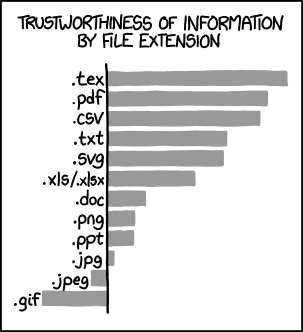
\includegraphics[width=0.47\textwidth]{figs/file_extensions.png}

  % *Every* figure should have a descriptive caption.
  \caption{On the trustworthiness of \LaTeX. Image courtesy of \texttt{xkcd}.}

  % The label is a handle you create so that you can refer to this
  % figure (using the \ref{} command) from other parts of your
  % document. LaTeX automatically renumbers figures and updates
  % references when you recompile, so you should do it this way rather
  % than hard-coding in references. Notice that I've also been
  % creating labels for the various sections in the document; I could
  % use \ref{} command to refer to those sections using their labels
  % too.
  \label{fig:tex}

\end{figure}

\subsection{Creating Tables}
\label{subsec:tables}

Again, refer to \texttt{results.tex} to learn how to create simple
tables (like table~\ref{tab:example}).
\begin{figure}[htb]
  \centering % centers the entire table

  % The following line sets the parameters of the table: we'll have
  % three columns (one per 'c'), each
  % column will be centered (hence the 'c'; 'l' or 'r' will left or
  % right justify the column) and the columns
  % will have lines between them (that's the purpose of the |s between
  % the 'c's).
  \begin{tabular}{|c|c|c|} 
    \hline \hline % draws two horizontal lines at the top of the table
    Column 1 & Column 2 & Column 3 \\ % separate column contents using the &
    \hline % line after the column headers
    $1$ & $3.1$ & $2.7$ \\
    $42$ & $-1$ & $1729$\\
    \hline \hline
  \end{tabular}

  % As with figures, *every* table should have a descriptive caption
  % and a label for ease of reference.
  \caption{An example table.}
  \label{tab:example}

\end{figure}



\section{Conclusions}
\label{sec:concl}

In this section, briefly summarize your paper --- what problem did you
start out to study, and what did you find? What is the key result /
take-away message? It's also traditional to suggest one or two avenues
for further work, but this is optional.


\section{Contributions}
\label{sec:contrib}

L.H. and M.C. paired programmed the scikit-learn python package.
L.H. ran the ridge regression and lasso experiments and M.C.
processed the csv files and created the graphs in the results. 
M.C. wrote the abstract and the introduction. L.H. wrote the background
and experiments. M.C and L.H. wrote the data preparation section. M.C. wrote the results. Both proofread the entire document and added input to each section.


\section{Acknowledgements} 
\label{sec:ack} 

This section is optional. But if there are people you'd like to thank for their help with the project --- a person who contributed some insight, friends who volunteered to help out with data collection, etc. --- then this is the place to thank them. Keep it short!


% This creates the references section. Open the project1.bib file to
% see how to organize your references.
\bibliography{project1}
\bibliographystyle{aaai} % sets citation and bib style, do not modify

\end{document}

\message{ !name(main.tex) !offset(-92) }
